% =====================================================================
% BBL514E Term Project --- Final Presentation
% A Three-Stage Hierarchical Soft-Fusion Framework
%   for Cryptocurrency Trading Signal Classification
%
% Authors: O.C. Yurutken (707251003)  C. Bilgin (504251013)  Y. Demirel (704252001)
% Build:   latexmk -xelatex presentation.tex
% =====================================================================

\documentclass[aspectratio=169,11pt]{beamer}
\usetheme{metropolis}

% --- fonts & encoding (xelatex) ----------------------------------------
\usepackage{fontspec}
\usepackage{polyglossia}
\setdefaultlanguage{english}

% --- core packages -----------------------------------------------------
\usepackage{graphicx}
\usepackage{booktabs}
\usepackage{multirow}
\usepackage{amsmath,amssymb}
\usepackage{xcolor}
\usepackage{tikz}
\usetikzlibrary{positioning,arrows.meta,calc,fit,backgrounds}
\usepackage{appendixnumberbeamer}

% --- ITU navy accent ---------------------------------------------------
\definecolor{itunavy}{HTML}{003366}
\definecolor{ituaccent}{HTML}{4B6E96}
\definecolor{lightgrey}{HTML}{E8ECF0}
\definecolor{darkgrey}{HTML}{4A4A4A}

\setbeamercolor{normal text}{fg=black, bg=white}
\setbeamercolor{alerted text}{fg=itunavy}
\setbeamercolor{example text}{fg=itunavy!80}
\setbeamercolor{frametitle}{bg=itunavy, fg=white}
\setbeamercolor{progress bar}{fg=itunavy}
\setbeamercolor{title separator}{fg=itunavy}
\setbeamercolor{progress bar in head/foot}{fg=itunavy, bg=lightgrey}
\setbeamercolor{progress bar in section page}{fg=itunavy}
\setbeamercolor{section title}{fg=itunavy}
\setbeamercolor{block title}{bg=itunavy, fg=white}
\setbeamercolor{block body}{bg=lightgrey, fg=black}
\setbeamercolor{itemize item}{fg=itunavy}
\setbeamercolor{itemize subitem}{fg=ituaccent}
\setbeamercolor{enumerate item}{fg=itunavy}

\setbeamertemplate{frametitle}[default][center]
\metroset{progressbar=frametitle,
          subsectionpage=progressbar,
          numbering=fraction,
          block=fill}

% --- figures path -----------------------------------------------------
\graphicspath{{../paper/figures/}}

% --- title page meta --------------------------------------------------
\title{A Three-Stage Hierarchical Soft-Fusion Framework\\for Cryptocurrency Trading Signal Classification}
\subtitle{BBL514E Pattern Recognition --- Term Project}
\author{Özgün Can Yürütken \and Çağatay Bilgin \and Yusuf Demirel}
\institute{%
  \footnotesize
  Department of Computer Engineering\\
  Istanbul Technical University
}
\date{May 2026}

% --- handy macros ------------------------------------------------------
\newcommand{\hl}[1]{\textcolor{itunavy}{\textbf{#1}}}
\newcommand{\fnote}[1]{{\scriptsize\textit{#1}}}

% =====================================================================
\begin{document}

% ---------------------------------------------------------------------
% SLIDE 1 --- Title
% ---------------------------------------------------------------------
\maketitle
\note{%
Good morning. We're presenting a three-stage hierarchical framework for
crypto Buy/Hold/Sell classification --- a pattern-recognition problem
where the decision is decomposed into three nested sub-problems.
I'm Özgün; with me are Çağatay and Yusuf.
}

% ---------------------------------------------------------------------
% SLIDE 2 --- Problem & Contributions
% ---------------------------------------------------------------------
\begin{frame}{Problem \& Contributions}

\textbf{Why is direct Buy/Hold/Sell classification hard?}
\begin{itemize}
\item Crypto is non-stationary; regimes shift on macro shocks.
\item Flat classifiers learn \alert{idiosyncratic} relationships that fail across regimes.
\end{itemize}

\vspace{2pt}
\textbf{Our approach.} Decompose the decision hierarchically:
\begin{enumerate}
\item \hl{Stage 1} --- local trend (ZigZag-labelled)
\item \hl{Stage 2} --- macro regime (rule-based FSM)
\item \hl{Stage 3} --- signal head that \alert{soft-fuses} the upstream posteriors
\end{enumerate}

\vspace{2pt}
\textbf{Three contributions:}
\begin{itemize}
\item A fully ablated 3-stage soft-fusion pipeline (BTC + ETH).
\item An \alert{asset-specific architecture finding} (no-free-lunch).
\item Hold-aware trading rules turn F1\,$=\,0.37$ into \alert{Sharpe\,$=\,1.15$}.
\end{itemize}
\end{frame}
\note{%
Crypto markets are noisy and non-stationary, so monolithic Buy/Hold/Sell
classifiers fail to generalise. We decompose the decision: first identify
the local trend, then the macro regime, then the trade.
Three contributions --- a fully ablated 3-stage pipeline, an asset-specific
architecture finding, and Hold-aware trading rules that recover Sharpe
1.15 despite frame-level F1 of only 0.37.
[Hand over to Çağatay for the data and Stage 1.]
}

% ---------------------------------------------------------------------
% SLIDE 3 --- Dataset & Stage 1 Design
% ---------------------------------------------------------------------
\begin{frame}{Dataset \& Stage 1 Design}
\small
\begin{columns}[T,onlytextwidth]
\column{0.50\textwidth}
\textbf{Data}
\begin{itemize}\setlength{\itemsep}{0pt}
\item BTC 2014--2025 (4{,}094 d), ETH 2017--2025 (3{,}060 d)
\item 22 macro covariates (Yahoo + FRED) with publication-release lags
\item \hl{Zero look-ahead leakage}, asserted in code
\end{itemize}

\vspace{2pt}
\textbf{Stage 1 label} --- ZigZag, $10\%$ dev., $\geq 15$-d seg.
\begin{itemize}\setlength{\itemsep}{0pt}
\item Classes: \emph{uptrend} / \emph{range} / \emph{downtrend}
\item 14 causal features \fnote{(RSI, MACD, ADX, \%B, ATR, OBV, log-returns)}
\end{itemize}

\column{0.48\textwidth}
\centering

\includegraphics[width=\linewidth,height=0.42\textheight,keepaspectratio]{fig_zigzag_lookahead.png}\\[-2pt]
{\footnotesize ZigZag label is \alert{revisable}.\\
106 causal cutoffs vs.\ offline label: \hl{42\%} disagree $\Rightarrow$ ML classifier needed.}
\end{columns}
\end{frame}
\note{%
We use daily BTC and ETH from Yahoo, plus 22 macroeconomic covariates from
FRED aligned with their real publication-release lags so there's no leakage.
The Stage-1 label comes from a ZigZag pivot detector. But the ZigZag label
is retrospective. When we recomputed it monthly using only past data, 42\%
of cutoff dates disagreed with the offline label. So we train an ML
classifier on 14 causal indicators; the model gives us a stable posterior
the rule cannot.
}

% ---------------------------------------------------------------------
% SLIDE 4 --- Stage 1 Results
% ---------------------------------------------------------------------
\begin{frame}{Stage 1 Results --- Frame F1 understates segment quality}
\small
\begin{columns}[T,onlytextwidth]
\column{0.42\textwidth}
\textbf{Optuna-tuned best per asset}
\begin{itemize}\setlength{\itemsep}{0pt}
\item Random Forest wins both
\item BTC: F1$_{\text{m}}$ \hl{0.563}, AUC \hl{0.76}
\item ETH: F1$_{\text{m}}$ \hl{0.571}, AUC \hl{0.75}
\end{itemize}
\fnote{All 8 tuned configs cleared F1 $\geq 0.50$ gate.}

\vspace{4pt}
\textbf{\alert{Segment-level finding}} (20-d rolling mode):
\begin{itemize}\setlength{\itemsep}{0pt}
\item Majority-vote consistency = \hl{0.77} BTC, \hl{0.83} ETH
\item In-segment dominant-class match $>$\,\hl{80\%}
\end{itemize}

\column{0.55\textwidth}
\centering

\includegraphics[width=\linewidth,height=0.66\textheight,keepaspectratio]{fig_stage1_truth_vs_pred_btc.png}\\[-2pt]
{\footnotesize Stage-1 BTC ground-truth vs.\ predicted (Random Forest, tuned).}
\end{columns}
\end{frame}
\note{%
Random Forest wins Stage 1 on both assets --- macro-F1 around 0.57 and
AUC 0.75. The more interesting result is segment-level: with rolling-mode
smoothing the model captures the macro trend structure 77--83\% of the
time even though its frame-level F1 is 0.57. This will matter again at
Stage 3.
[Back to Özgün for Stage 2.]
}

% ---------------------------------------------------------------------
% SLIDE 5 --- Stage 2: Composite Macro FSM
% ---------------------------------------------------------------------
\begin{frame}{Stage 2 --- Composite Macro Finite-State Machine}
\small
\begin{columns}[T,onlytextwidth]
\column{0.40\textwidth}
\textbf{Why a rule-based FSM?}\\
\fnote{Unsupervised approaches first tried and rejected:}
\begin{itemize}\setlength{\itemsep}{0pt}
\item K-Means: failed on 2008 GFC
\item Constrained K-Means: noisy
\item HMM: unstable transitions
\item GMM: 2024--25 \alert{stickiness}
\end{itemize}

\vspace{2pt}
\textbf{FSM design}
\begin{itemize}\setlength{\itemsep}{0pt}
\item 8 rules + 1 re-entry guard
\item 5 macro features \fnote{(VIX z, yield-curve, $\Delta$VIX, DXY z, M2 YoY)}
\item Output: $\hat p_{\text{regime}} + \tau_t$
\end{itemize}
\fnote{Fires on '08 GFC, '20 COVID, '22 bear, '25 tariff bear.}

\column{0.57\textwidth}
\centering

\includegraphics[width=\linewidth,height=0.78\textheight,keepaspectratio]{fig_stage2_fsm.png}\\[-2pt]
{\footnotesize Regime timeline (Bear / Neutral / Bull) over S\&P\,500, BTC, ETH.}
\end{columns}
\end{frame}
\note{%
Stage 2 emits the macro regime. We didn't pick a rule-based FSM by default
--- we first tried K-Means, semantic-constrained K-Means, HMM, and a GMM.
All failed on the 2008 crisis or showed unstable transitions. So we
engineered an 8-rule FSM with VIX hysteresis, minimum dwell times, and a
yield-curve guard. It correctly identifies every major bear since 2008,
including the 2025 tariff bear. Stage 2's output is a one-hot regime plus
a tenure scalar.
}

% ---------------------------------------------------------------------
% SLIDE 6 --- Stage 3 Soft-Fusion Architecture
% ---------------------------------------------------------------------
\begin{frame}{Stage 3 --- Soft-Fusion Architecture}

\textbf{Soft fusion} --- pass the \alert{full posterior vectors}, not hard labels:

\vspace{-2pt}
\begin{equation*}
z_t = \big[\,\hat p_{\text{trend}}(t),\;\hat p_{\text{trend}}^{(\text{smooth-10})}(t),\;\hat p_{\text{regime}}(t),\;\tau_t,\;o_t\,\big] \in \mathbb{R}^{16}
\end{equation*}

\vspace{-4pt}
\begin{columns}[T,onlytextwidth]
\column{0.36\textwidth}
\fnote{$o_t$: 6 oscillators \\(RSI, MACD, \%B, ATR, CCI, WilliamsR).}

\vspace{4pt}
\fnote{Label (causal):}
\vspace{-6pt}
\[
\hspace{-6pt}\scalebox{0.78}{$y_t = \begin{cases}\text{Buy} & \text{if }\tfrac{P_{t+5}-P_t}{P_t} > k\hat\sigma_t\\[1pt]\text{Sell} & \text{if }\tfrac{P_{t+5}-P_t}{P_t} < -k\hat\sigma_t\\[1pt]\text{Hold} & \text{otherwise}\end{cases}$}
\]
\fnote{$\hat\sigma_t$: 20-d past-only rolling $\sigma$; $k=0.5$.}

\column{0.62\textwidth}
\centering
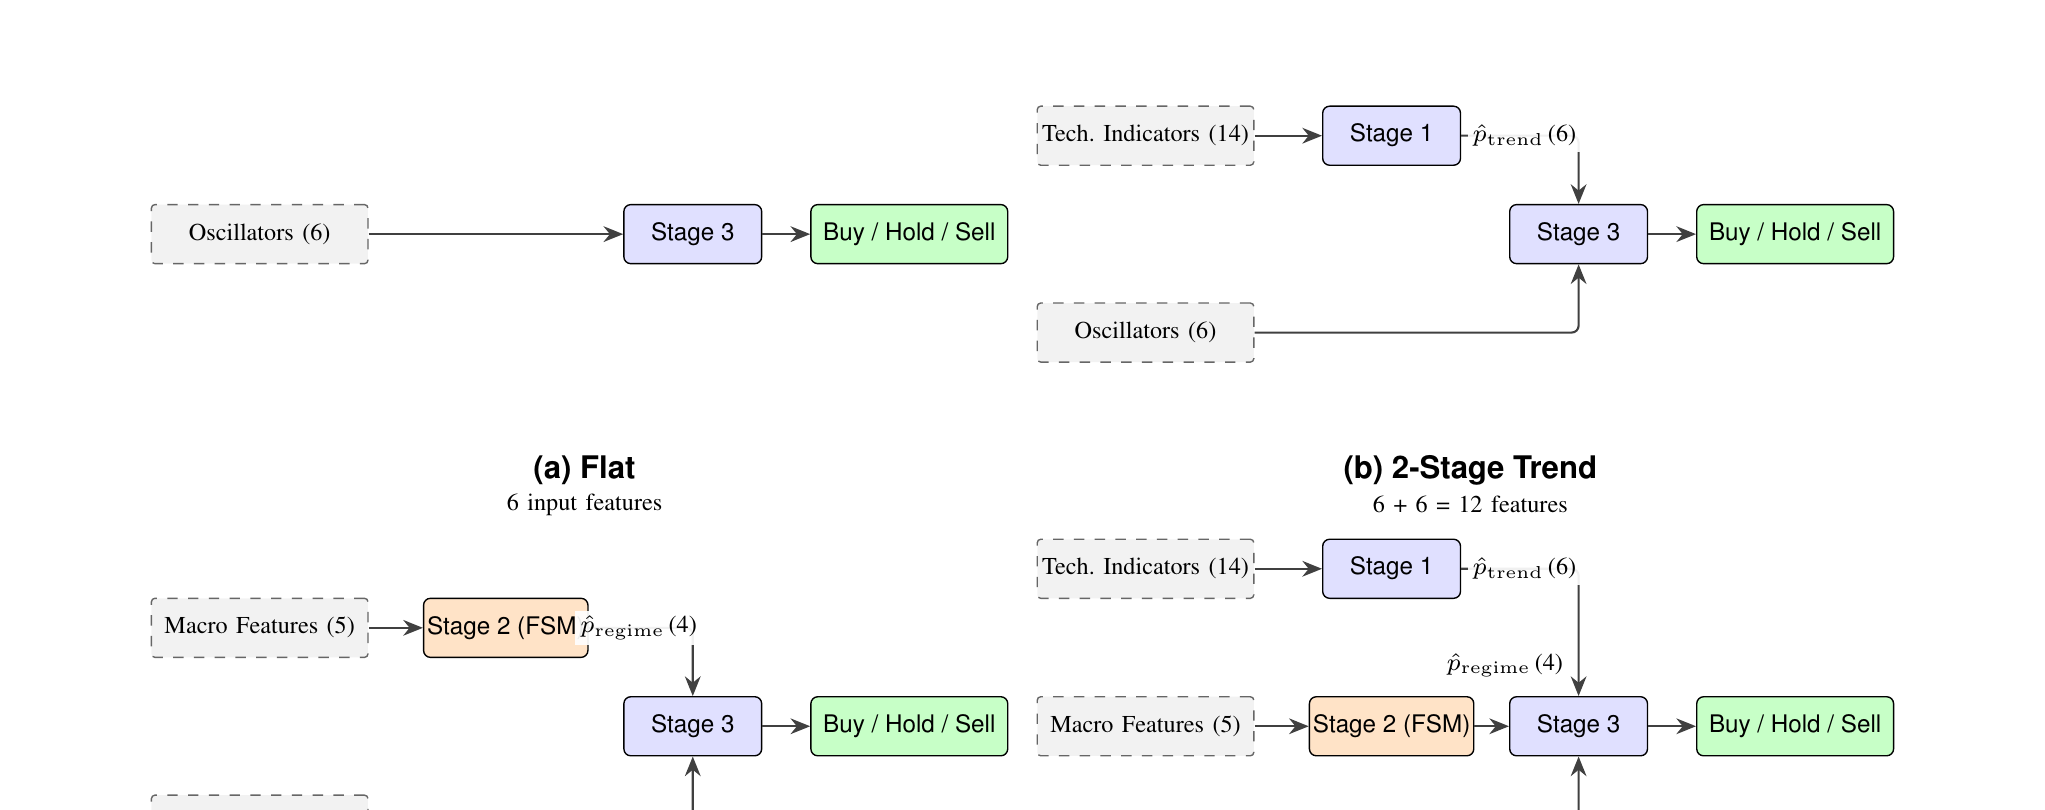
\includegraphics[width=\linewidth]{fig_arch_diagram.png}\\[-2pt]
{\scriptsize Four architectures ablated: Flat $\to$ 2-Stage Trend $\to$ 2-Stage Macro $\to$ 3-Stage Full.}
\end{columns}
\end{frame}
\note{%
Stage 3 is where everything fuses. We pass the full probability vector
from Stage 1, not the hard class --- that's the ``soft'' in soft fusion.
Together with the regime one-hot, regime tenure, and six oscillators we
get a 16-dimensional input. The label is a causal adaptive threshold ---
5-day forward return against a 20-day rolling volatility, no look-ahead.
To isolate where value comes from, we ablate four architectures: flat
baseline, two 2-stage variants, and the full 3-stage.
[Yusuf will run us through the experiments.]
}

% ---------------------------------------------------------------------
% SLIDE 7 --- Experimental Setup
% ---------------------------------------------------------------------
\begin{frame}{Experimental Setup --- Walk-Forward + Optuna}
\small
\begin{columns}[T,onlytextwidth]
\column{0.54\textwidth}
\textbf{Outer CV} --- expanding-window walk-forward
\begin{itemize}\setlength{\itemsep}{0pt}
\item Val window $v=200$\,d; advance by $v$ (non-overlap).
\item Gap $g=10$\,d $>$ label horizon $h=5$\,d $\Rightarrow$ \alert{no leakage}.
\item Folds: BTC 16/12 (S1/S3); ETH 10/6.
\end{itemize}

\vspace{2pt}
\textbf{Inner CV} --- 5-fold walk-forward for Optuna
\begin{itemize}\setlength{\itemsep}{0pt}
\item Folds span regimes: 2017, 2019, 2021, 2023, 2025.
\item TPE + MedianPruner, 30 trials per model/stage.
\end{itemize}

\vspace{2pt}
\textbf{Backtest} --- 0.1\% one-way cost; 3 rules:
\fnote{stateful $\cdot$ defensive reset $\cdot$ prob.-weighted.}

\column{0.44\textwidth}
\centering
\begin{tikzpicture}[
  every node/.append style={font=\tiny\sffamily},
  fold/.style={draw=itunavy, fill=itunavy!18, minimum height=3mm, inner sep=0pt},
  test/.style={draw=itunavy, fill=itunavy, minimum height=3mm, inner sep=0pt},
  gap/.style={draw=darkgrey, fill=lightgrey, minimum height=3mm, inner sep=0pt}
]
\foreach \i/\trw in {0/10, 1/14, 2/18, 3/22} {
  \node[fold, minimum width=\trw mm, anchor=west] (tr\i) at (0.7, -\i*0.45) {};
  \node[gap,  minimum width=3 mm, anchor=west] (gp\i) at (tr\i.east) {};
  \node[test, minimum width=4 mm, anchor=west] (te\i) at (gp\i.east) {};
  \node[anchor=east, font=\tiny] at (0.55, -\i*0.45) {f\the\numexpr\i+1\relax};
}
\node[font=\tiny\itshape] at (2.3,0.4) {train $\cdot$ gap $\cdot$ test};
\end{tikzpicture}\\[-3pt]
{\scriptsize Expanding-window: $g=10$\,d, $v=200$\,d.}

\vspace{8pt}
\hl{1\,h\,43\,m} full ablation\\(M3 MacBook Air)\\[2pt]
\fnote{4 archs $\times$ 4 models $\times$ 2 assets $\times$ 30 trials.}
\end{columns}
\end{frame}
\note{%
All evaluation is expanding-window walk-forward with a 10-day gap larger
than the 5-day label horizon to prevent leakage. The inner walk-forward
for Optuna spans five historical regimes so hyperparameters don't overfit
a single bull or bear period. Sixteen outer folds for BTC, ten for ETH.
Four classifiers, four architectures, two assets, 0.1\% transaction cost.
The full ablation runs in under two hours on a laptop.
}

% ---------------------------------------------------------------------
% SLIDE 8 --- Architecture Ablation
% ---------------------------------------------------------------------
\begin{frame}{Architecture Ablation --- The Asset-Specific Optimum}
\centering
{\footnotesize
\setlength{\tabcolsep}{4pt}
\renewcommand{\arraystretch}{1.0}
\begin{tabular}{@{}llrrrr@{}}
\toprule
Asset & Architecture \fnote{(best $\langle$rule, model$\rangle$)} & Sharpe & Return & MaxDD & F1$_{\text{m}}$\\
\midrule
BTC & Flat \fnote{(state., xgb)}           & 0.93 & +1565\% & --75\% & 0.349\\
BTC & 2-Stage Trend \fnote{(probw., lgbm)}  & 1.08 & +539\%  & --28\% & 0.347\\
BTC & 2-Stage Macro \fnote{(state., rf)}    & 0.98 & +1606\% & --53\% & 0.356\\
BTC & \hl{\textbf{3-Stage Full}} \fnote{\textbf{(state., xgb)}} & \hl{\textbf{1.15}} & \hl{\textbf{+2901\%}} & \hl{\textbf{--46\%}} & \hl{\textbf{0.367}}\\
BTC & Buy \& Hold                           & 0.95 & +2972\% & --77\% & ---\\
\midrule
ETH & \hl{\textbf{Flat}} \fnote{\textbf{(probw., lgbm)}} & \hl{\textbf{0.52}} & \hl{\textbf{+26\%}} & \hl{\textbf{--18\%}} & 0.347\\
ETH & 2-Stage Trend \fnote{(defens., xgb)}  & 0.39 & +43\%   & --55\% & 0.361\\
ETH & 2-Stage Macro \fnote{(state., mlp)}   & 0.47 & +69\%   & --51\% & 0.343\\
ETH & 3-Stage Full \fnote{(probw., lgbm)}   & 0.34 & +19\%   & --18\% & 0.350\\
ETH & Buy \& Hold                           & 0.26 & \alert{--7\%} & --72\% & ---\\
\bottomrule
\end{tabular}}

\vspace{6pt}
\begin{columns}[T,onlytextwidth]
\column{0.30\textwidth}
\small\textbf{BTC:} every hierarchical variant beats Flat $\Rightarrow$ hierarchy adds value.
\column{0.30\textwidth}
\small\textbf{ETH:} Flat beats 3-Stage $\Rightarrow$ hierarchy \alert{overfits} the shorter 5-yr history.
\column{0.36\textwidth}
\small\begin{block}{No-free-lunch}
\footnotesize Depth is \alert{asset-specific}. Validate per asset and per dataset size.
\end{block}
\end{columns}
\end{frame}
\note{%
Here's our headline finding. For BTC, every hierarchical variant beats
the flat baseline, and the full 3-stage hits Sharpe 1.15 --- versus 0.95
for Buy \& Hold, with the drawdown cut from 77\% to 46\%.
For ETH the relationship reverses: the flat 6-oscillator model wins, and
adding upstream posteriors actually degrades Sharpe. We attribute this
to ETH's shorter history --- five years versus ten for BTC --- which
makes the higher-dimensional model overfit.
The practical takeaway: no-free-lunch. Every hierarchical proposal must
be re-validated per asset.
}

% ---------------------------------------------------------------------
% SLIDE 9 --- Equity Curves
% ---------------------------------------------------------------------
\begin{frame}{Equity Curves --- The Money Slide}
\centering

\includegraphics[width=0.82\linewidth,keepaspectratio,height=0.62\textheight]{fig_arch_equity.png}\\[-2pt]
{\scriptsize Best architecture per ablation vs.\ Buy \& Hold. BTC (top), ETH (bottom).}

\vspace{2pt}
\begin{columns}[T,onlytextwidth]
\column{0.49\textwidth}
{\footnotesize\textbf{BTC} --- 3-Stage Full pulls ahead in the \hl{2022 bear} via Hold-class abstention. Drawdown: 77\% $\to$ \hl{46\%}.}
\column{0.49\textwidth}
{\footnotesize\textbf{ETH} --- B\&H \alert{loses 7\%}; every architecture beats it. Hold class as a \hl{risk filter} $\Rightarrow$ F1\,$=\,0.37$ yields Sharpe\,$=\,1.15$.}
\end{columns}
\end{frame}
\note{%
The equity curves tell the story. On BTC the 3-Stage Full curve pulls
away from Buy \& Hold during the 2022 bear because the model abstains
via the Hold class. On ETH, where Buy \& Hold actually loses 7\% over
the test span, our framework returns +26\%.
The Hold class is the secret --- it's a risk filter that converts low
frame accuracy into high economic precision.
}

% ---------------------------------------------------------------------
% SLIDE 10 --- Key Takeaways
% ---------------------------------------------------------------------
\begin{frame}{Key Takeaways}
\vfill
\begin{block}{1.\ Frame $\neq$ Trade}
Macro-F1 $0.37$, AUC $0.53$ \quad$\Longrightarrow$\quad \hl{Sharpe $1.15$} via Hold-aware rules.
\end{block}

\begin{block}{2.\ Architecture is asset-specific}
3-Stage wins BTC; Flat wins ETH. \alert{No universal hierarchy in financial ML.}
\end{block}

\begin{block}{3.\ Reproducible}
Walk-forward CV $+$ Optuna $+$ Docker. Code, OOF predictions, FastAPI demo all public.
\end{block}
\vfill
\centering\large
\textbf{$\Rightarrow$ Now the live demo.}
\end{frame}
\note{%
Three takeaways.
One --- frame-level metrics under-report trade-level value when a Hold class
is available; F1 0.37 yields Sharpe 1.15.
Two --- architectural depth is asset-specific, an explicit no-free-lunch
result.
Three --- everything is reproducible: one Docker container, FastAPI back-end,
Chart.js front-end.
[Over to Yusuf for the live demo.]
}

% ---------------------------------------------------------------------
% SLIDE 11 --- Demo Handoff
% ---------------------------------------------------------------------
\begin{frame}[plain]
\vfill
\centering
{\Huge\textbf{\textcolor{itunavy}{Live Demo}}}\\[12pt]
{\large FastAPI back-end \;\textbullet\; Chart.js front-end \;\textbullet\; one Docker container}\\[10pt]
{\large \texttt{http://localhost:8000}}\\[24pt]
{\small\itshape Stage 1 posterior \;$\to$\; Stage 2 regime \;$\to$\; Stage 3 signal \;$\to$\; equity curve}
\vfill
\end{frame}
\note{%
I'll spin up the Docker container and walk through a live BTC prediction:
asset selector, real-time inference showing the three intermediate
posteriors, then the equity-curve comparison versus Buy \& Hold, and
finally a quick toggle to ETH to confirm the asset-specific finding.
}

\end{document}
